\subsection{Oppgave 6}
\label{section:oppgave6}
For denne oppgaven har vi valgt å lage en 3-D animasjon av T-nøkkelen som roterer. Nærmere bestemt, så har vi implementert 3D-animasjon for de $3$ numeriske metodene vi har brukt til å løse systemet, nemlig Eulers metode, RK4 og RK45.

\subsubsection{Punktgenerering}
Før vi animerer løsningene $X$ fra oppgave $5$, så genererer vi alle løsningene $X$, og serialiserer disse slik at vi kan kjøre animasjonene så mange ganger vi vil uten å måtte generere alle punktene på nytt. Alt vi da trenger å gjøre er å laste opp punktene til grafikkinterfacet, og vi kan se animasjonene umiddelbart. Punktgenereringa blir kjørt med steglengde er $0.005.$ med $0\leq t \leq 500\text{ s}.$ Den dynamiske kontrollen av stegstørrelse som ble diskutert i forrige oppgave blir også brukt her. Denne kontrollen har vært viktig for at energien ikke endrer seg nevneverdig. Implementasjonen for punktgenereringen ligger i "kode/oppgave6/punktgenerering.py".

\subsubsection{Animasjon av T-nøkkel}
For å animere løsningene fra oppgave $5$ som ni funksjoner av tiden, så har vi valgt å bruke biblioteket PyOpenGL. PyOpenGL er en Python binding til OpenGL og relaterte APIer \cite{PYOPENGL:1}. Vi har valgt å bruke dette biblioteket fordi det blir lettere og ikke minst raskerer å integrere animasjonen av T-nøklene med resten av koden vi har skrevet i Python og NumPy. Vi kan for eksempel endre stegstørrelsen vi bruker i vår implementasjon av RK45, og denne endringen vil reflekteres i animasjonen uten at vi trenger å gjøre ekstra arbeid.\newline\newline
Måten systemet vårt for animasjon er satt opp i to deler, punktgenerering og animasjon. Koden for punktgenereringen finnes i "kode/oppgave6/punktgenerering.py" og her approksimeres X(t) med en gitt steglengde og intervall med alle de implementerte numeriske metodene for alle oppgavene. Etter de er generert dumpes dataen i filer slik at de kan brukes senere. Det som dumpes for hver numeriske metode er en liste med W-matriser som representerer X(t) og en like lang liste med korresponderende t-verdier. \newline\newline Animasjonsdelen ligger i "kode/oppgave6/animasjon.py" og her brukes den genererte dataen for å animere t-nøkkelen. Origo for X(t) representerer punktet det stive legemet roterer om, altså massesenteret. For å tegne t-nøkkelen riktig har vi derfor kalkulert hvor massesenteret burde være på legemet og tegnet nøklene med tanke på dette. I hvert bilde i animasjonen av én t-nøkkel tegnes det to sylindere. Den korteste sylinderen i t-nøkkelen tegnes langs den første søylevektoren i X(t). Den lengste sylinderen, altså håndtaket tegnes parallelt med den andre søylevektoren i X(t). Slik ligger da t-nøkkelen til enhver tid på flaten generert av de to første søylevektorene, med Massesenteret til nøkkelen i origo på X(t). I systemet tegnes t-nøkkelen basert på tid, slik at simulasjonen stemmer. Vi bruker listen med t-verdier og tid som har gått siden starten av animasjonen sammen med W-matrisene vi får fra punktgenerasjonen og kalkuler riktig index på W. I koden ser dette slik ut: \newline 
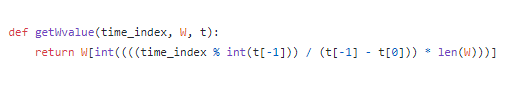
\includegraphics{rapport/resultat/bilder/get_w_value.PNG}
\newline
Her er "timeIndex" antall sekunder siden start og ved hjelp av modulusregningen vil dette da loope over intervallet vi har spesifisert.\newline\newline
Under følger animasjonene av løsningene $X$ til oppgave $5$ a, b, og c.

\subsubsection{Animasjon av T-nøkkel fra oppgave 5a}
\label{subseq:oppgavea}
\href{https://youtu.be/mxFFCeYBHsw}{https://youtu.be/mxFFCeYBHsw}\newline\newline 
YouTube-videoen ovenfor viser rotasjon av $3$ T-nøkler med $X(t)$ for\newline $\vec{\omega}(0)=\begin{bmatrix}1&0.05&0\end{bmatrix}.$ Den røde T-nøkkelen (T-nøkkelen nærmest origo i koordinatsystemet) representerer $X(t)$ når den er løst med RK45, den grønne T-nøkkelen (T-nøkkelen i midten) representerer $X(t)$ når den er løst med RK4, og den blå T-nøkkelen (T-nøkkelen lengt fra origo i koordinatsystemet) representerer $X(t)$ når den er løst med Eulers Metode. Som vi kan se, så har alle T-nøklene ustabil rotasjon her. Rundt $3:03$ i videoen, så ser vi at T-nøklene løst med RK4 og RK45 begynner å rotere om sin $z$-akse. Disse rotasjonene kommer til å bli diskutert i mer detalj i Kapittel \ref{section:diskusjon}.

\subsubsection{Animasjon av T-nøkkel fra oppgave 5b}
\label{subseq:oppgaveb}
\href{https://youtu.be/IKKG5pIe50I}{https://youtu.be/IKKG5pIe50I}\newline\newline
YouTube-videoen ovenfor viser rotasjon av $3$ T-nøkler med $X(t)$ for\newline $\vec{\omega}(0) = \begin{bmatrix}0 & 1 & 0.05 \end{bmatrix}$. Her ser vi at T-nøklene roterer med relativt stabil rotasjon i starten, men rotasjonen blir ustabil for alle T-nøklene jo lenger de har rotert. Denne ustabile rotasjonen er ikke like ekstrem som den fra animasjonen ovenfor, men likevel nevneverdig. Dette vil også bli diskutert i Kapittel \ref{section:diskusjon}.

\subsubsection{Animasjon av T-nøkkel fra oppgave 5c}
\label{subseq:oppgavec}
\href{https://youtu.be/yUi333x3vd8}{https://youtu.be/yUi333x3vd8}\newline\newline
YouTube-videoen ovenfor viser rotasjon av $3$ T-nøkler med $X(t)$ for\newline $\vec{\omega}(0) = \begin{bmatrix}0.05 & 0 & 1 \end{bmatrix}$. Her ser vi at rotasjonen er stabil $\forall t\geq 0.$ Hvorfor er det slik at rotasjonen er stabil her, og ikke for de andre initialbetingelsene for $\omega$? Det kommer vi til å diskutere i Kapittel \ref{section:diskusjon}. 